\section{Mechanik strömender Fluide}
\begin{auf}
    286
\end{auf}
Durch ein Rohr, bestehend aus zwei Teilstücken mit unterschiedlichem Querschnitt, die sich in verschiedenen Höhenlagen befinden, fließt Wasser (Dichte $\varrho=10^3\frac{kg}{m^3}$). Teilstück 1 hat den Durchmesser $D_1=9cm$, und der (statische) Druck in ihm beträgt $p_1=250kPa$. Im Teilstück 2 mit dem Durchmesser $D_2=20cm$, welches $\Delta h=15m$ höher liegt, soll der Druck $p_2=110kPa$ betragen.
\begin{enumerate}
    \item[a] Wie groß sind die Strömungsgeschwindigkeiten $v_1$ und $v_2$ in den beiden Teilstücken?
    \item[b] Wie groß sind Volumenstrom $I$ und Gesamtdruck $p_{ges}$ im Rohr?
\end{enumerate}
\begin{figure}[h]
    \centering
    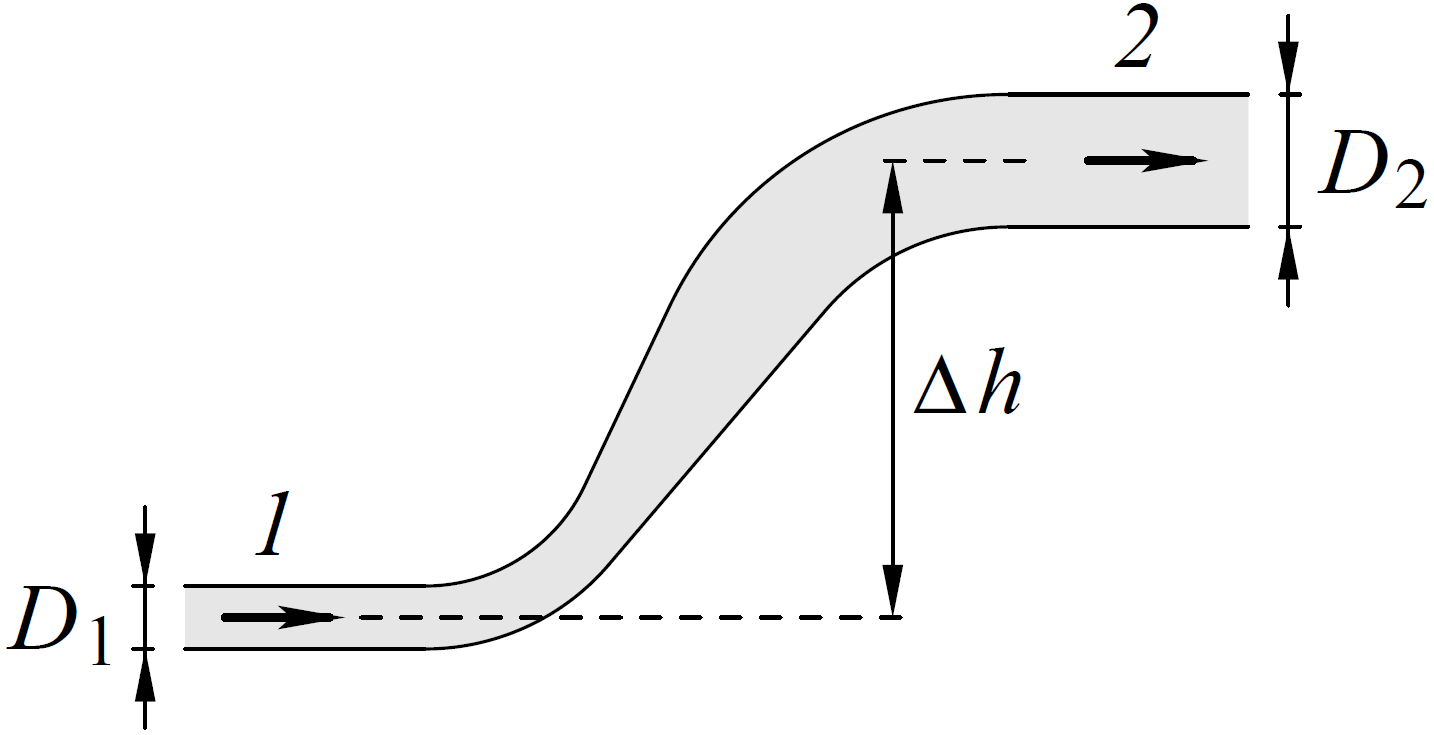
\includegraphics[width=0.7\linewidth]{images/286_0.png}
    \caption{Versuchsaufbau Aufgabe 286}
\end{figure}
Für beide Höhenniveaus $h_1=0$ und $h_2=\Delta h$ gilt die Bernoulli-Gleichung, wonach in beiden Teilstücken des Rohres der Gesamtdruck $p_{ges}$, das heißt die Summe aus statischem Druck (Kolbendruck) $p$, dynamischem Druck (Staudruck) $\frac{\varrho}{2}v^2$ und Schweredruck $\varrho\cdot g\cdot h$, gleich ist.
\begin{align}
    p_{ges}=p_1+\frac{\varrho}{2}v_1^2=p_2+\frac{\varrho}{2}v_2^2+\varrho\cdot g\cdot\Delta h	\label{eq:286_bernoulli}
\end{align}
Desweiteren gilt für die Volumenstromstärke $I$ in den beiden Querschnitten $A_1$ und $A_2$ die Kontinuitätsgleichung.
\begin{align}
    I=v_1\cdot A_1=v_2\cdot A_2	\label{}
\end{align}